\documentclass[11pt,fleqn]{article}

\setlength {\topmargin} {-.15in}
\setlength {\textheight} {8.6in}

\usepackage{amsmath}
\usepackage{amssymb}
\usepackage{color}
\usepackage{tikz}
\usetikzlibrary{automata,positioning,arrows}
\usepackage{diagbox}



\newcommand{\be}{\begin{enumerate}}
\newcommand{\ee}{\end{enumerate}}

\begin{document}

\textbf{Exercise 4.1.18:}: The girth of a graph is the length of its shortest cycle. If a graph is acyclic, then its
girth is infinite. Add a method girth() to GraphProperties that returns the girth of
the graph. Hint : Run BFS from each vertex. The shortest cycle containing s is a shortest
path from s to some vertex v, plus the edge from v back to s.\\

\textbf{Solution:}\\
\begin{center}
	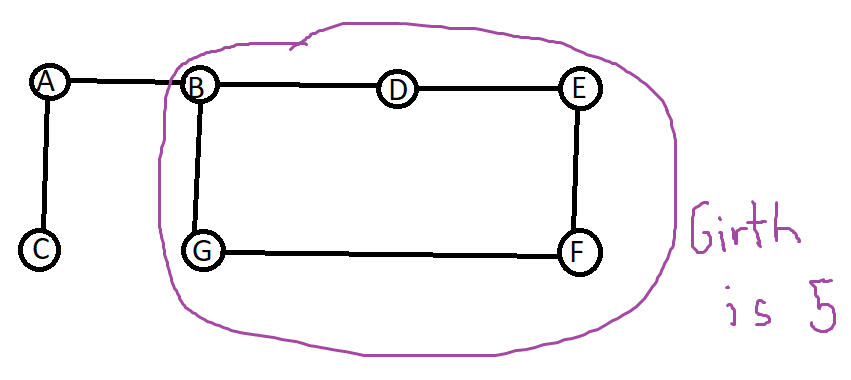
\includegraphics[scale=0.7]{4.1.18.png}
\end{center}
BFS can find/detect a cycle as it goes down a layer. It see/checks if something previously has been marked. If so, then cycle is formed.\\

BFS\_cycle: Detect and calculate length of cycle.

OUT: A\\
Queue: $A_\phi,B_A,C_A,D_B,G_B,E_D,F_G$\\
Dequueing E, we find already marked but not yet Dequeued. So we know $E-F$ is part of the cycle



	


\end{document}
